\section{Algorithm}
Let $M$ denote the mesh model, and let S denote the Laplacian skeleton. We propose an algorithm for partitioning S into a minimum set of nice (disjoint) subgraphs, each of which can be fabricated in a 3D printer without using support structures. Decomposing S into two pieces can be done by duplicating a node v and splitting the arcs incident to $v$ properly; however, decomposing $M$ around $v$ requires the determination of the position and normal of a cutting plane; to realize these and guarantee a nice look on the finished surface with shortest seams, we set a constraint of minimizing the peripheral length of a cut.
For realizing the objectives, in addition to the angle constraint for the arcs, we need to consider the dimension constraint: the dimension of the printing model should be within the working space of a given 3D printer.

To summarize, our objectives are the minimization of (1) the number of partitioned components $N$; (2) the total peripheral length of each cut $L_i$, i.e., $\Sigma L_i$.

The constraints of the problem are as follows:
(1) Each arc of the partitioned subgraph subtends to an axis by an angle of no larger than $\theta$, where $\theta$ is defined based on printing experiments without using any support structure. This guarantees that the corresponding mesh component is support-free during the printing process.
(3) Let the normal direction of the cut $c$ (pointing to the exterior of the partitioned part) be denoted as $n(c)$; as the directed arcs of $H_i$ are translated to a common origin, they form a fork, the fork has a central ray, which is the middle axis of the minimum cone that encloses the fork, let $Cone(H_i)$ be the cone, let the central ray of $Cone(H_i)$ be denoted as $r(H_i)$; in order to guarantee support-free fabrication for the boundary of the cut, the angle between $n(c)$ and $r(H_i)$ should satisfy $A(n(c), r(Hi)) �� \pi/2 + \theta$.
(3) The base of a printing model should be large enough to gather sticky force from the building platform, such that the model is not deformed during the building process. Formally, let $b(H_i)$ denote the area of the base of the mesh component corresponding to $H_i$, let $\tau$ be a user-defined threshold value., then we have $b(H_i) \geq \tau$. Here $\tau$ can be determined by some simple printing experiments.
(4) Each cut partitions a single subgraph.

To summarize, we have the following optimization system:

	Objective: min $N$ and min$\sum(L_i)$ 	(1)
	Subject to: $A(e, r(H_i)) �� \theta$, for each $e \in H_i$	(2)
	$A(n(c), r(H_i)) \leq \pi/2+ \theta$	(3)
	$b(H_i) \geq \tau $	(4)
	$c \cap S = c \cap H_i$	(5)
where $H_i$ is the target subgraph to be cut off.


Assume that we are given a function $TirmBFS(v, G)$ which traverses $G$ from $v$ in a breath first search manner until all arcs satisfying constraints (2-3) are determined, we have the following algorithm for skeleton decomposition. The main idea of our algorithm is to randomly search the graph using Monte Carlo Method, which randomly chooses a node of $S$ to start traversing and randomly chooses an arc of the current node as the exit path.

\begin{algorithm}
\caption{Algorithm: $SkeletonMeshDecomposition(S, M)$}
\label{alg:Framwork}
\begin{algorithmic}[1]
\REQUIRE~
The Laplacian skeleton $S$ of a mesh model $M$;
\ENSURE~
The decomposition of $S$ into a set of the least pieces of subgraphs $T$, each arc of which subtends to an axis by an angle of no larger than $\theta$;
\STATE $T = \emptyset$; $min = \inf$; $count$ = 0; $max-iter$ = a user defined large constant;
\WHILE {$count < max-iter$}
\STATE  $G=S$; $U= \emptyset$;
\WHILE {$G\neq \emptyset$}
\FOR{($i=1$; $i<| S |$; $i++$ )}
\STATE $H = TrimBFS(v_i, S, \theta)$;
\STATE $H = S / H$;
\STATE $U = U \cup H$;
\IF {$| U | < min$}
\STATE $T = U$;
\STATE  $min = | U | $;
\ENDIF
\ENDFOR
\ENDWHILE
\STATE $count =count + 1$;
\ENDWHILE
\label{code:fram:select} \\
\RETURN $T$;
\end{algorithmic}
\end{algorithm}


Skeleton Partition:
Next we shall show how $TirmBFS(v, S, \theta)$ works to find a maximal subgraph starting at $v$ that satisfies the angle constraint. Let $H$ be the current subgraph obtained. When an arc $e$ of $G$ is visited, we need to determine whether it should be included into $H$. If the start of each outgoing arc of $H$ is moved to a common site, then the arcs form a fork (Figure \ref{fig:sphere}). A naive method to judge whether $e$ should be included is to move the start of $e$ to the origin of the fork, and compute the angle between $e$ and each arc of the fork, $e$ is included if the maximum angle between $e$ and each arc of the fork does not exceed $0.5\pi$. However, this method would require $O(K^2)$ time, where $K$ is the number of the nodes of $S$. To speed up this process, we keep the pair of vectors hat form the largest angle and judge whether a new vector expands the mouth of the fork; if so, determine the other vector (may not be an arc of $H$). See Figure \ref{fig:sphere}, let $\hat{e_i}$  and $\hat{e_j}$ be the units of these two vectors obtained so far. For simplicity, we denoted by $F( \hat{e_i}, \hat{e_j} )$ the fork with the starts of all unit vectors converging at the origin of the coordinate frame, where $\hat{e_i}$  and  $\hat{e_j}$  are the pair of unit vectors that form the largest angle in the fork. Let $\hat{e_k}$  be the unit of a new vector to be processed next, if $\hat{e_k}$ penetrates through the blue circle, then no change need to be made to the fork; otherwise, let $D_{i,j}$ denote the spherical disk that passes through the endpoints of $\hat{e_i}$  and $\hat{e_j}$ whose central axis is collinear with $\hat{e_i}$  + $\hat{e_j}$, let $c_{i,j}$ be the center of $D_{i,j}$, let $B_{i,j}$ be the boundary circle of $D_{i,j}$. The circle passing through $\hat{e_k}$  and $c_{i,j}$, denoted as $O( \hat{e_k}, c_{i,j})$, intersects  $B_{i,j}$ at two points, let $q$ the point further away from the endpoint of $\hat{e_k}$, then $\overrightarrow{oq}$ and $\hat{e_k}$ are the two extreme vectors that to be used in the next iteration. To summarize,
A new arc $e_k$ is taken by Function $TirmBFS$ if and only if one of the following two conditions is met:
(1) the angle between $\overrightarrow{oc_{i,j}}$ and $\hat{e_k}$, denoted as $A(\overrightarrow{oc_{i,j}}, \hat{e_k})$, satisfies  $A(\overrightarrow{oc_{i,j}}, \hat{e_k}) \leq A(\overrightarrow{oc_{i,j}}, \hat{e_i})$;
(2) $A(\overrightarrow{oc_{i,j}}, \hat{e_k})  \leq \pi - 2\theta$, where $q = O( \hat{e_k}, c_{i,j}) \cap B_{i,j}$.

\begin{figure}[tbp]
  \centering
  \mbox{} \hfill
  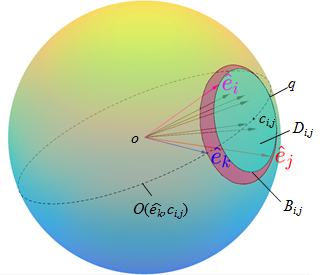
\includegraphics[width=0.4\textwidth]{figs/take_arc.png}
  \caption{\label{fig:sphere}%
           Illustration of unit vectors, unit sphere, spherical disks, and the determination of taking a new edge in $TrimBFS$.}
\end{figure}

Mesh Partition:

[Anton: Optimization of cutting sequence]



Although the skeleton partition tells us a rough sketch of the mesh partition, i.e., the cutting plane should be in the vicinity of each node $v$ incident to two distinct subgraphs. Yet we need to determine the exact positions of the cutting planes. For each node $v$ that is incident to at least two distinct subgraphs $H_i$ and $H_j$, we process it using the following cutting principle:

The Cutting Scheme for $M$:
See Figure \ref{fig:fillets}, at the position of node $v$, define two fillets each of which contains all planes that orthogonal to the vectors in $Cone(H_i)$ or $Cone(H_j)$, let $Fillet(H_i)$ and $Fillet(H_j)$ be the two fillets respectively. Depending on the relative position of $Fillet(H_i)$ and $Fillet(H_j)$, we have the following cases:


$Fillet(H_i) \cap Fillet(H_j) / {v} \neq \emptyset$


See Figure \ref{fig:fillets}(a) for an illustration of the case. To address the issue, we shall randomly sample a set of cutting planes from $Fillet(H_i) \cap Fillet(H_j) / {v}$, and determine the one achieving the minimum cutting length.


$Fillet(H_i) \cap Fillet(H_j) = {v}$


See Figure \ref{fig:fillets}(b). In this case, two cuts $c_1$ and $c_2$ are inevitable in order to separate the mesh, however, care must be taken as the angle between $c_1$ and $c_2$ should be constrained by $A(n(c_1), n(c_2)) \leq \pi/2+ \theta$. If this constraint is violated, one more cut in between $c_1$ and $c_2$ is required; while the base of each partitioned component should be constrained by $b(H_i) \geq \tau$ and $b(H_j) \geq \tau$. If any of the constraints is not satisfied, we shall translate the fillets along the build direction in an opposite sense until the constraints are satisfied (See Figure fillets). In this process, if the translation hits an

\begin{figure}[tbp]
  \centering
  \mbox{} \hfill
  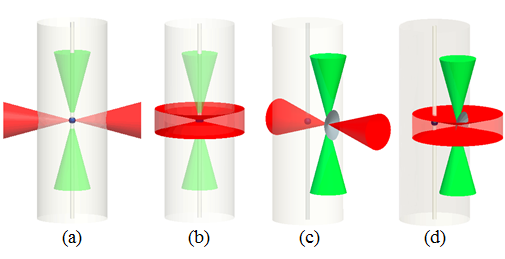
\includegraphics[width=0.5\textwidth]{figs/fillets.png}
  \caption{\label{fig:fillets}%
           Illustration of fillets: (a)two fillets with their apexes coinciding at a node of $S$ share an intersection zone; (b)two fillets with their apexes coinciding at a node of $S$ share a single point; (c) two fillets with their apexes coinciding at a concave vertex of $R_v$ share an intersection zone; (d) two fillets with their apexes coinciding at a concave vertex of $R_v$ share the concave vertex only. The two fillets are marked by red and green colors respectively.}
\end{figure}


Let $R(v)$ be the set of concave vertices on M that are incident to v during the Laplacian shrinking process, we shall truncate $R(v)$ such that the non-significant concave vertices are removed away. Here, given a vertex vi and any of its neighbor $v_j$, $v_i$ is concave if $(v_i - v_j)(n_j - n_i)$ is nonnegative, the significance of a concave vertex can be quantified as the magnitude of $(v_i - v_j)(n_j - n_i)$ \cite{au2012mesh}.
See Figure \ref{fig:fillets}(c-d), for each vertex in $R(v)$, we shall process a pair of fillets as done for node $v$ above. Particularly, if $v$ is neighbor to at least three nodes in $S$ while is only neighbored to a single node $w$ in subgraph $H_i$, then the separation of the mesh component corresponding to $H_i$ may not be feasible if only $R(v)$ is used, this is because the position of $v$ is designed for the purpose of connecting the different branches. To separate the mesh component of $H_i$, we process arc $vw$ as follows:
Given a user-defined threshold value $\delta$, if $| vw | \leq \delta$, then $R(v)$ is extended to contain the concave vertices of $M$ that are incident to $w$. On the other hand, if $| vw | > \delta$, then a partition of the arc $vw$ by an interval of $\delta$ is applied. Subsequently, for each node along the arc $vw$, the above scheme for processing a pair of fillets for node $v$ is exploited, see Figure \ref{fig:forward_tracing}.








Finally, if the cut-subgraph constraint (Eq. (5)) is violated, a sequence of iterative cutting is required.

\begin{figure}[tbp]
  \centering
  \mbox{} \hfill
  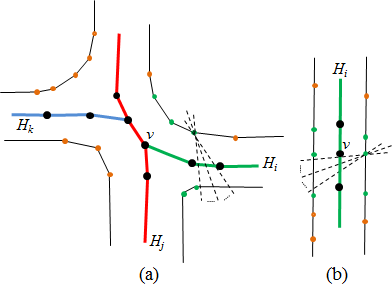
\includegraphics[width=0.4\textwidth]{figs/forward_tracing.png}
  \caption{\label{fig:forward_tracing}%
           2D illustration editing a long arc for cutting.}
\end{figure}


However, a split of the 1D skeleton cannot tell us the exact position of the cut on the mesh. Sometimes, it is possible for a piece of meat, i.e., a mesh component, that is not printable free of support even though its corresponding skeleton is printable free of support. This is because the skeleton piece that shares a junction node with any other subgraph may compromise its topology locally \cite{AuTCCL08}, and therefore cannot precisely describe the local topology feature of the partitioned meat. In this case, we shall regenerate the skeleton of the meat by running our skeleton partition algorithm on the meat, and then apply the $SkeletonMeshDecomposition$ Algorithm on it. Refer to Figure \ref{fig:arm} for an illustration.

\begin{figure}[tbp]
  \centering
  \mbox{} \hfill
  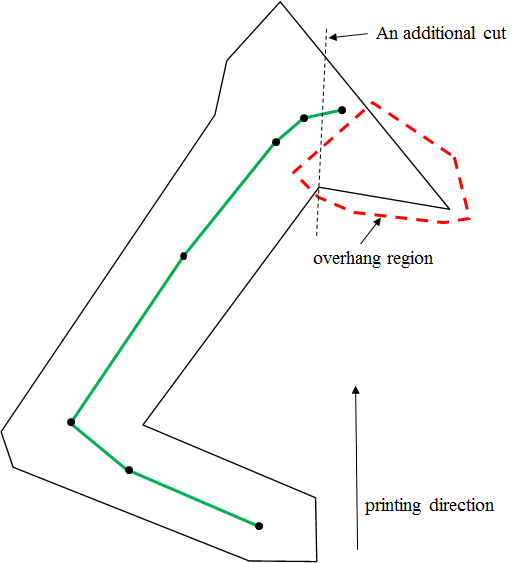
\includegraphics[width=0.45\textwidth]{figs/arm.png}
  \caption{\label{fig:arm}%
           Illustration of editing the mesh component of a printable subgraph:(a) A meat with an overhange that requires support; (b)Regeneration of the skeleton of the meat by $SkeletonMeshDecomposition$ Algorithm; (c) the partition result by $SkeletonMeshDecomposition$ Algorithm.}
\end{figure}

Cut-subgraph Intersection Detection: In order to take care of Eq. (7), the intersections of a cut and the subgraphs can be efficiently determined by taking advantage of the correspondence between the mesh vertices and the skeleton nodes: each vertex of $M$ is mapped to a single node of $S$. Therefore, as a cut goes through the mesh surface, the endpoints of the cut edges of $M$ lend us the information of the cut subgraphs. Approximately, if a cut $c$ goes into an edge whose endpoints are incident to a subgraph $H$, then $c$ cuts $H$.



\begin{algorithm}
\caption{Algorithm: $TirmBFS(v, S,\theta)$}
\label{alg:Framwork}
\begin{algorithmic}[1]
\REQUIRE~
A node $v$ of Laplacian skeleton $S$, an angular value $\theta$;
\ENSURE~
 A maximal subgraph $H$ rooted at $v$ and its corresponding mesh component that meet the constraints (Eq.2-5);
\STATE starting from $v$, initialize F($\hat{e_i}$, $\hat{e_j}$); $H = \emptyset $;
\WHILE  {the current arc $e_k$ of $S$ picked by the BFS process is nonempty}
  \IF  {$A(\overrightarrow{oc_{i,j}},  \hat{e_k}) \leq A(\overrightarrow{oc_{i,j}},  \hat{e_i})$}
  \STATE  $H = H \cup {e_k}$;
  \ENDIF
  \STATE $q = O( \hat{e_k}, c_{i,j}) \cap B_{i,j}$;
  \IF  {$A(\overrightarrow{oq},  \hat{e_k}) \leq \pi- 2\theta$}
  \STATE  $\hat{e_i}=  \hat{e_k}$;
  \STATE $\hat{e_j} =  \overrightarrow{oq}$;
  \STATE  update $B_{i,j}$ and $c_{i,j}$;
  \STATE  $H = H \cup {e_k}$;
  \ENDIF
\ENDWHILE
\STATE  call the cutting scheme for $M$;
\STATE  $M= M/M_H$;
\label{code:fram:select} \\
\RETURN  $H$ and $M_H$;
\end{algorithmic}
\end{algorithm}


In line 2 of $TirmBFS$, the BFS process randomly chooses an arc incident to $v$ to proceed on. In order to guarantee a greater chance of converging to the optimal result in a short time, we apply a training-and-learning procedure for the first 1000 runs. Formally, let $N_v$ be the number of times an arc is chosen as the exit arc when node $v$ is visited. Given the data of the first 1000 runs, as a node $v$ is visited, the probability of choosing an arc $e$ as an outgoing arc in the subsequent runs is,

	$P(v, e) = N_v/1000$	(7)

To further speed up the process of $Trim-BFS$, we assign a mark that stores the minimum number of subgraphs obtained so far, such that the current branching can be terminated if its output number of subgraphs is larger than the mark.

Since the traversing process assigns a specific direction to each arc that was originally undirected in $S$, it is not obvious whether the angle constraint is satisfied, To clarify this, we provide the following lemma.

Lemma 1: $H = Tirm_BFS(v, G, \theta)$ is a maximal subgraph of $G$ that satisfies the angle constraint, i.e., each arc of $H$ subtends to an axis by an angle of no larger than $\theta$.

Proof: Suppose to the contrary that $H$ violates the angle constraint, there exists a directed arc that does not satisfy the angle constraint. For example, arc $\vec a\quad\overrightarrow(c, a)$ or arc $\vec a\quad\overrightarrow(b, c)$ in Figure \ref{fig:proof}. Such case is impossible as Line 3 and Line 6 of function $Trim-BFS$ excludes any directed arc that violates the angle constraint of no larger than $\theta$ with respect to the (virtual) central axis.
It remains to prove that $H$ is maximal, i.e., the largest graph rooted at $v$ that covers all the arcs that satisfies the angle constraint. Suppose that this is not true, there must exist an arc that was mistakenly discarded due to the direction in which the arc is traversed. Let $(b, c)$ be one of such arcs, as illustrated in Figure \ref{fig:proof}(a). When the arc is directed from $b$ to $c$, it is not included as it violates the angle constraint, but can be included if the arc directed from $c$ to $b$. We shall prove in a case-by-case basis.
If $c$ is not reachable from $v$ via a directed path passing through $b$ (Figure \ref{fig:proof} (c)), then $c$ is only reachable from $b$, arc $bc$ should not be included and line 6 of Function $Trim-BFS$ correctly handle this case.
Otherwise, $c$ is reachable from $v$ via a directed path without passing through $b$ (Figure \ref{fig:proof} (d)). As $c$ is visited, by Line 2 of Function $Trim-BFS$, each arc leaving $c$ is considered, and $\vec a\quad\overrightarrow(c, b)$ is correctly included into $H$. This completes the proof. ��



\begin{figure}[tbp]
  \centering
  \mbox{} \hfill
  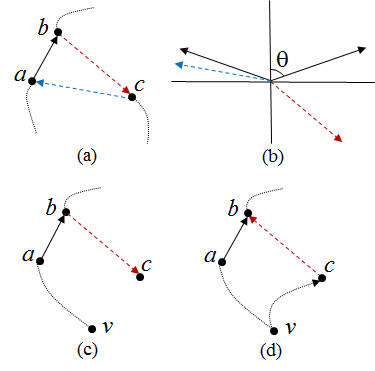
\includegraphics[width=0.4\textwidth]{figs/proof.png}
  \caption{\label{fig:proof}%
           Illustration of taking a directed arc into a maximal subgraph by $Trim-BFS$.}
\end{figure}
Figure WSX:




